\section{Empirical Grounding and Validation Protocol}
\label{sec:evidence}

We ground two architectural claims with released evidence. Task studies show
that bounded panel-and-synthesis policies can execute behind one model
interface. A separate planning case study estimates how routing structure changes
fleet capacity. These studies ground the execution and systems claims; they do
not establish the matched-budget scaling hypothesis posed in
Section~\ref{sec:required-experiments}.

\subsection{End-to-end multi-model execution}

The current public evaluation manifest\footnote{Versioned evaluation manifest:
\href{https://github.com/vllm-project/semantic-router/blob/84e7440cf523452c92cb742fca14cb50d27598d3/bench/router_flow/real_eval/current_eval_matrix.json}{github.com/vllm-project/semantic-router}.}
records summaries of the GPQA-Diamond and LiveCodeBench runs in
Table~\ref{tab:preliminary-evals}. Each invokes \texttt{vllm-sr/auto} through the
standard API \texttt{model} field, but uses a benchmark-specific constituent
pool, signal policy, topology, and response contract. The alias is therefore a
serving surface, not an immutable MoM identity. Router-side normalization is
applied where configured, and benchmark-native scoring treats failed or missing
items as incorrect. The tasks are GPQA-Diamond~\citep{rein_2023_gpqa} and the
January--April 2025 slice of LiveCodeBench~\citep{jain_2024_livecodebench}.

\paragraph{Accuracy-first composition.}
The two configurations spend a finite panel and synthesis budget rather than
minimizing active calls. They demonstrate an accuracy-first operating mode in
which the served object includes coordination and format handling, not merely
the final constituent call. Because the public benchmarks predate the evaluated
2026 constituents, these results characterize end-to-end system execution and
should not be read as contamination-free generalization.

\begin{table}[H]
\caption{Project-reported end-to-end runs in the versioned evaluation manifest
\citep{vllm_sr_2026_microagent}. Scores map each task's native metric to a
0--100 scale; workloads and active-call budgets differ across rows.}
\label{tab:preliminary-evals}
\centering
\footnotesize
\setlength{\tabcolsep}{4pt}
\begin{tabular}{L{0.19\linewidth}L{0.34\linewidth}L{0.11\linewidth}L{0.17\linewidth}L{0.05\linewidth}}
\toprule
Evaluation & Executed topology & Metric & Score (95\% Wilson CI) & $n$ \\
\midrule
GPQA-Diamond, formal-50 & Three parallel reasoning calls followed by synthesis &
Accuracy & 96.0 [86.5, 98.9] & 50 \\
LiveCodeBench v6, Jan.--Apr. 2025 & Risk-conditioned panel totaling four or six
calls, including synthesis & Pass@1 & 92.6 [87.7, 95.6] & 175 \\
\bottomrule
\end{tabular}
\vspace{2pt}

\begin{minipage}{0.96\linewidth}
\scriptsize
GPQA is the formal-50 run. LiveCodeBench retains a 175-item denominator and
counts five missing generations as failures. Wilson intervals reflect per-item
sampling uncertainty, not protocol, benchmark-exposure, or model stochasticity.
\end{minipage}
\end{table}

\begin{figure}[H]
  \centering
  \makebox[\textwidth][c]{%
    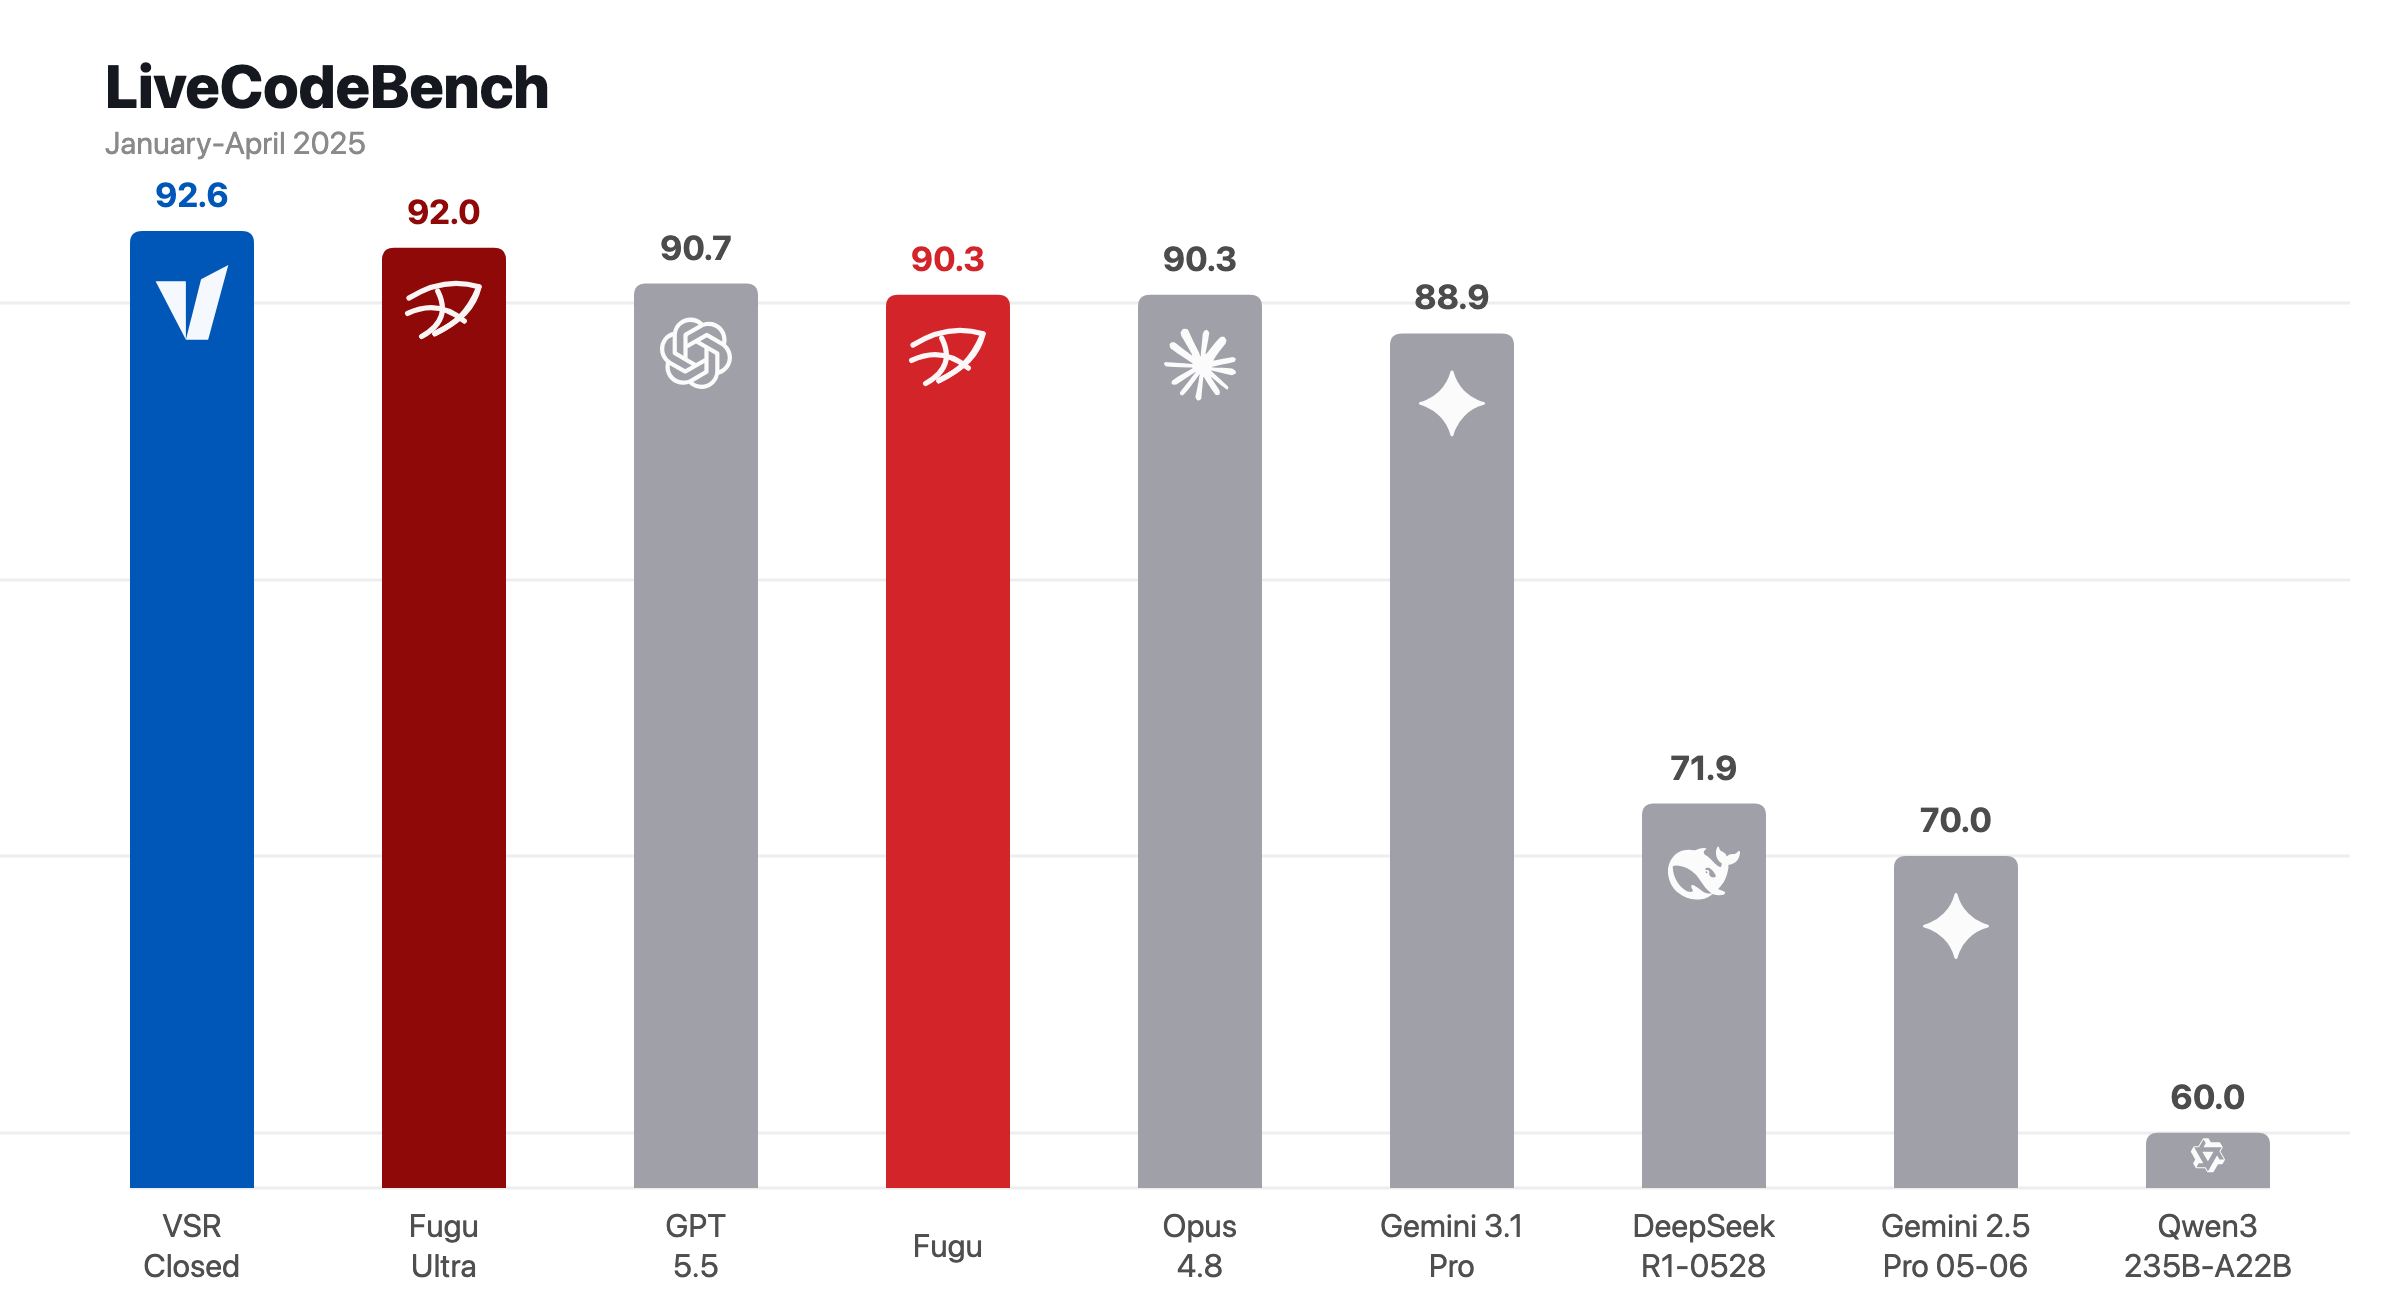
\includegraphics[width=0.27\paperwidth,trim=0 0 1080bp 0,clip]{figures/fig6_livecodebench_scorecard.png}%
    \hspace{0.03in}%
    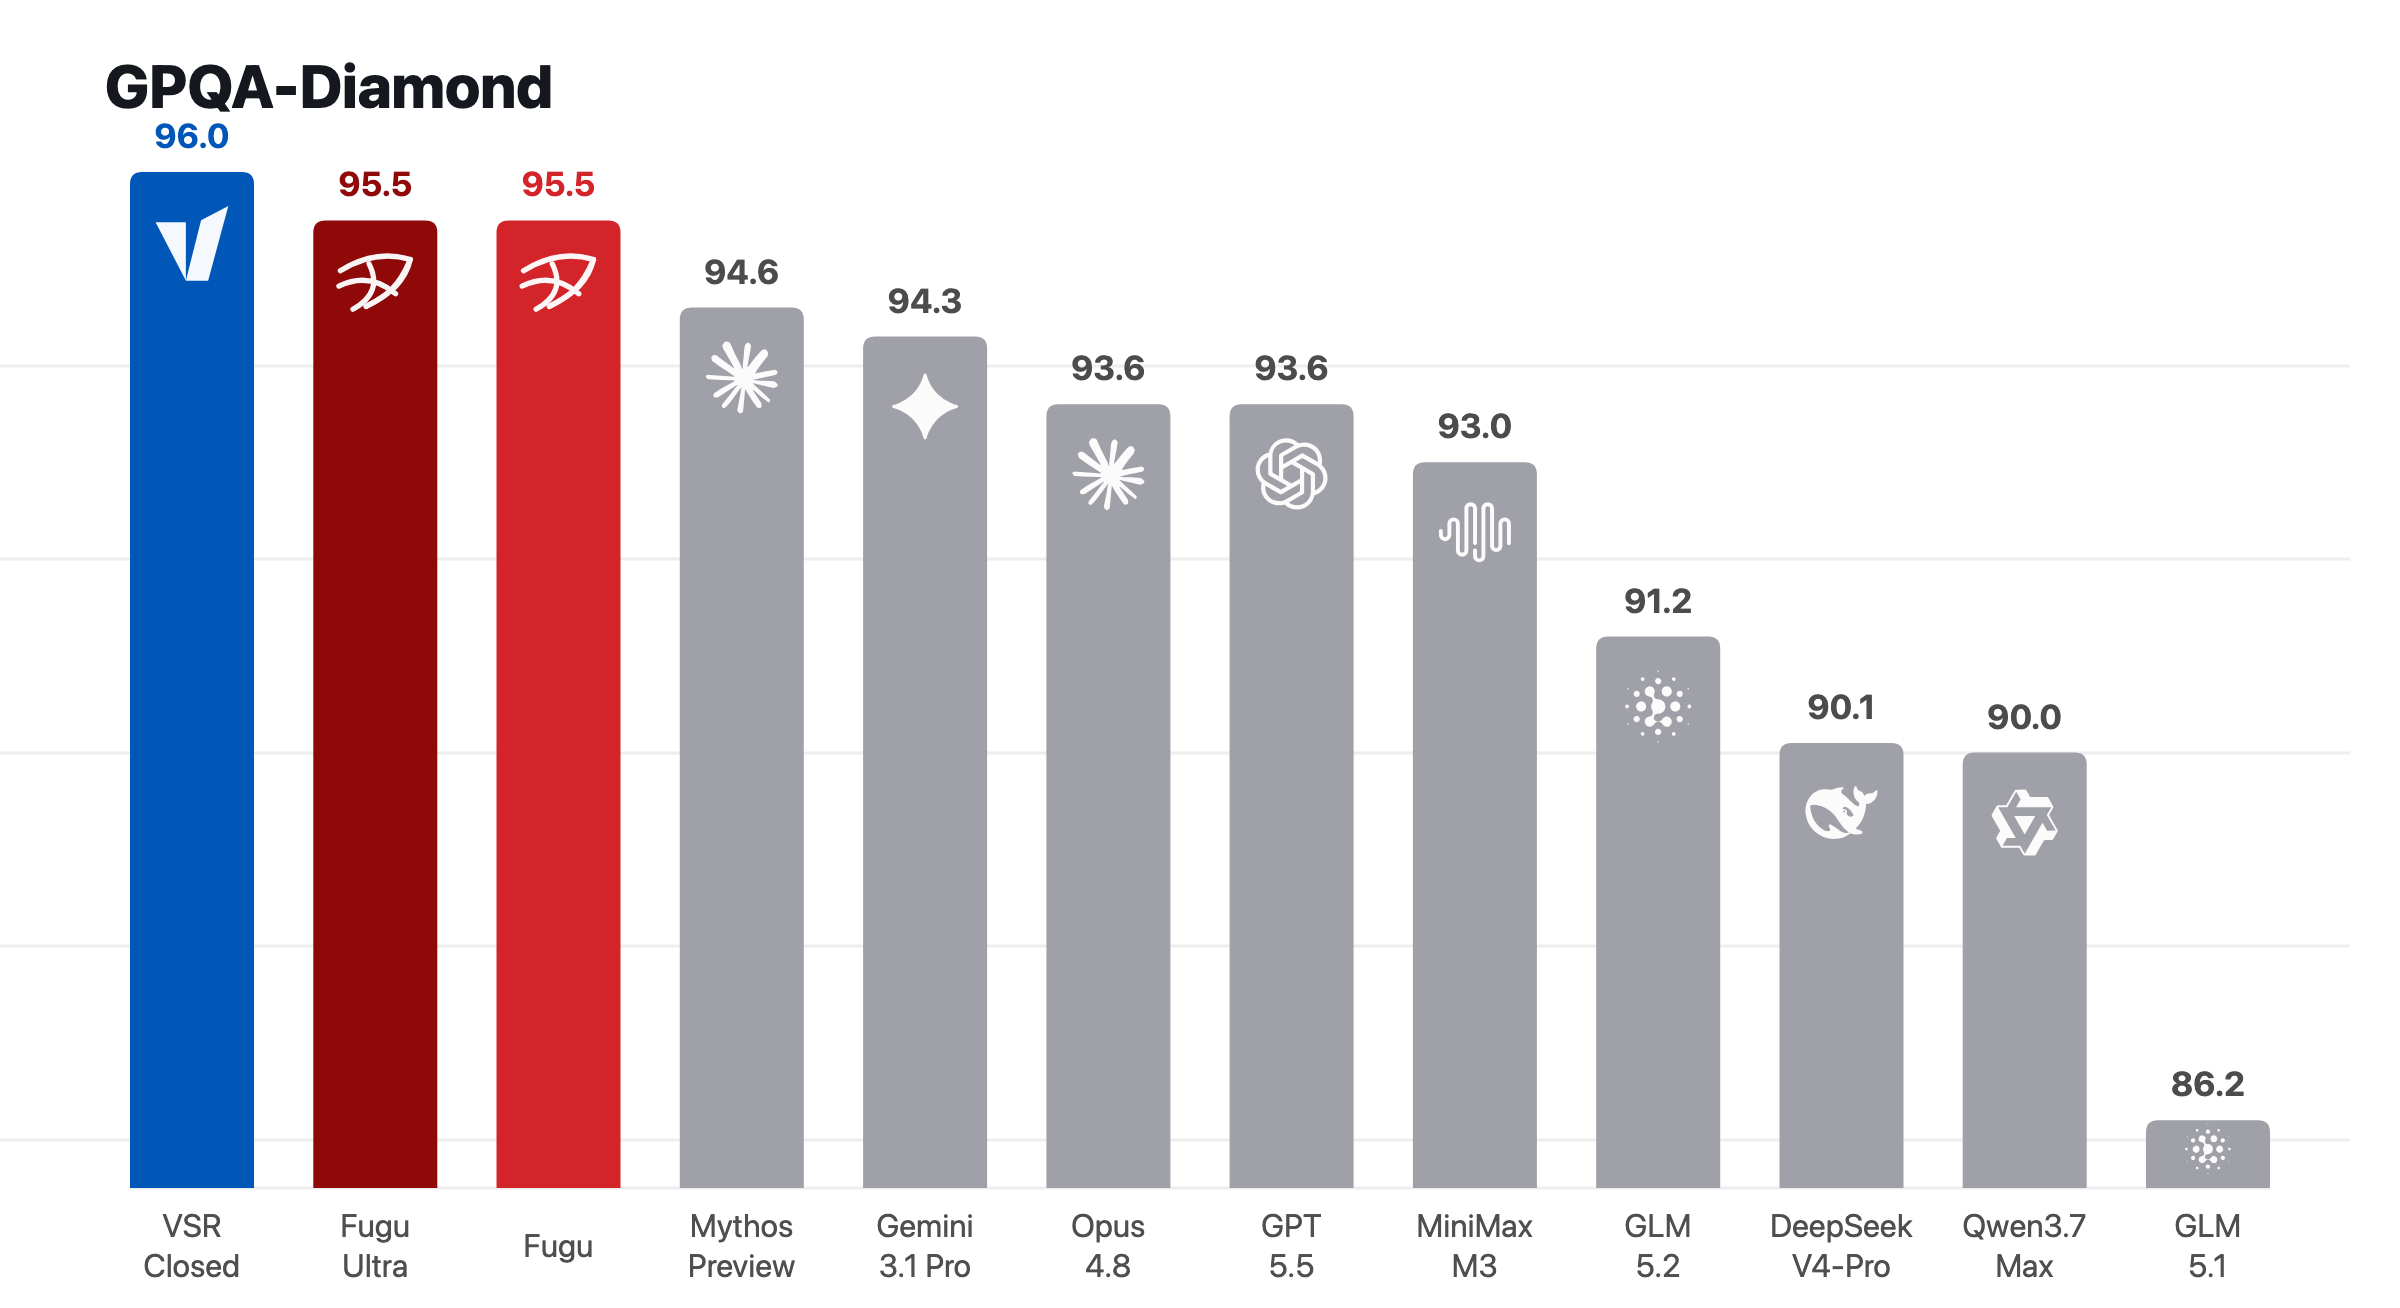
\includegraphics[width=0.27\paperwidth,trim=0 0 1035bp 0,clip]{figures/fig6_gpqa_scorecard.png}%
    \hspace{0.03in}%
    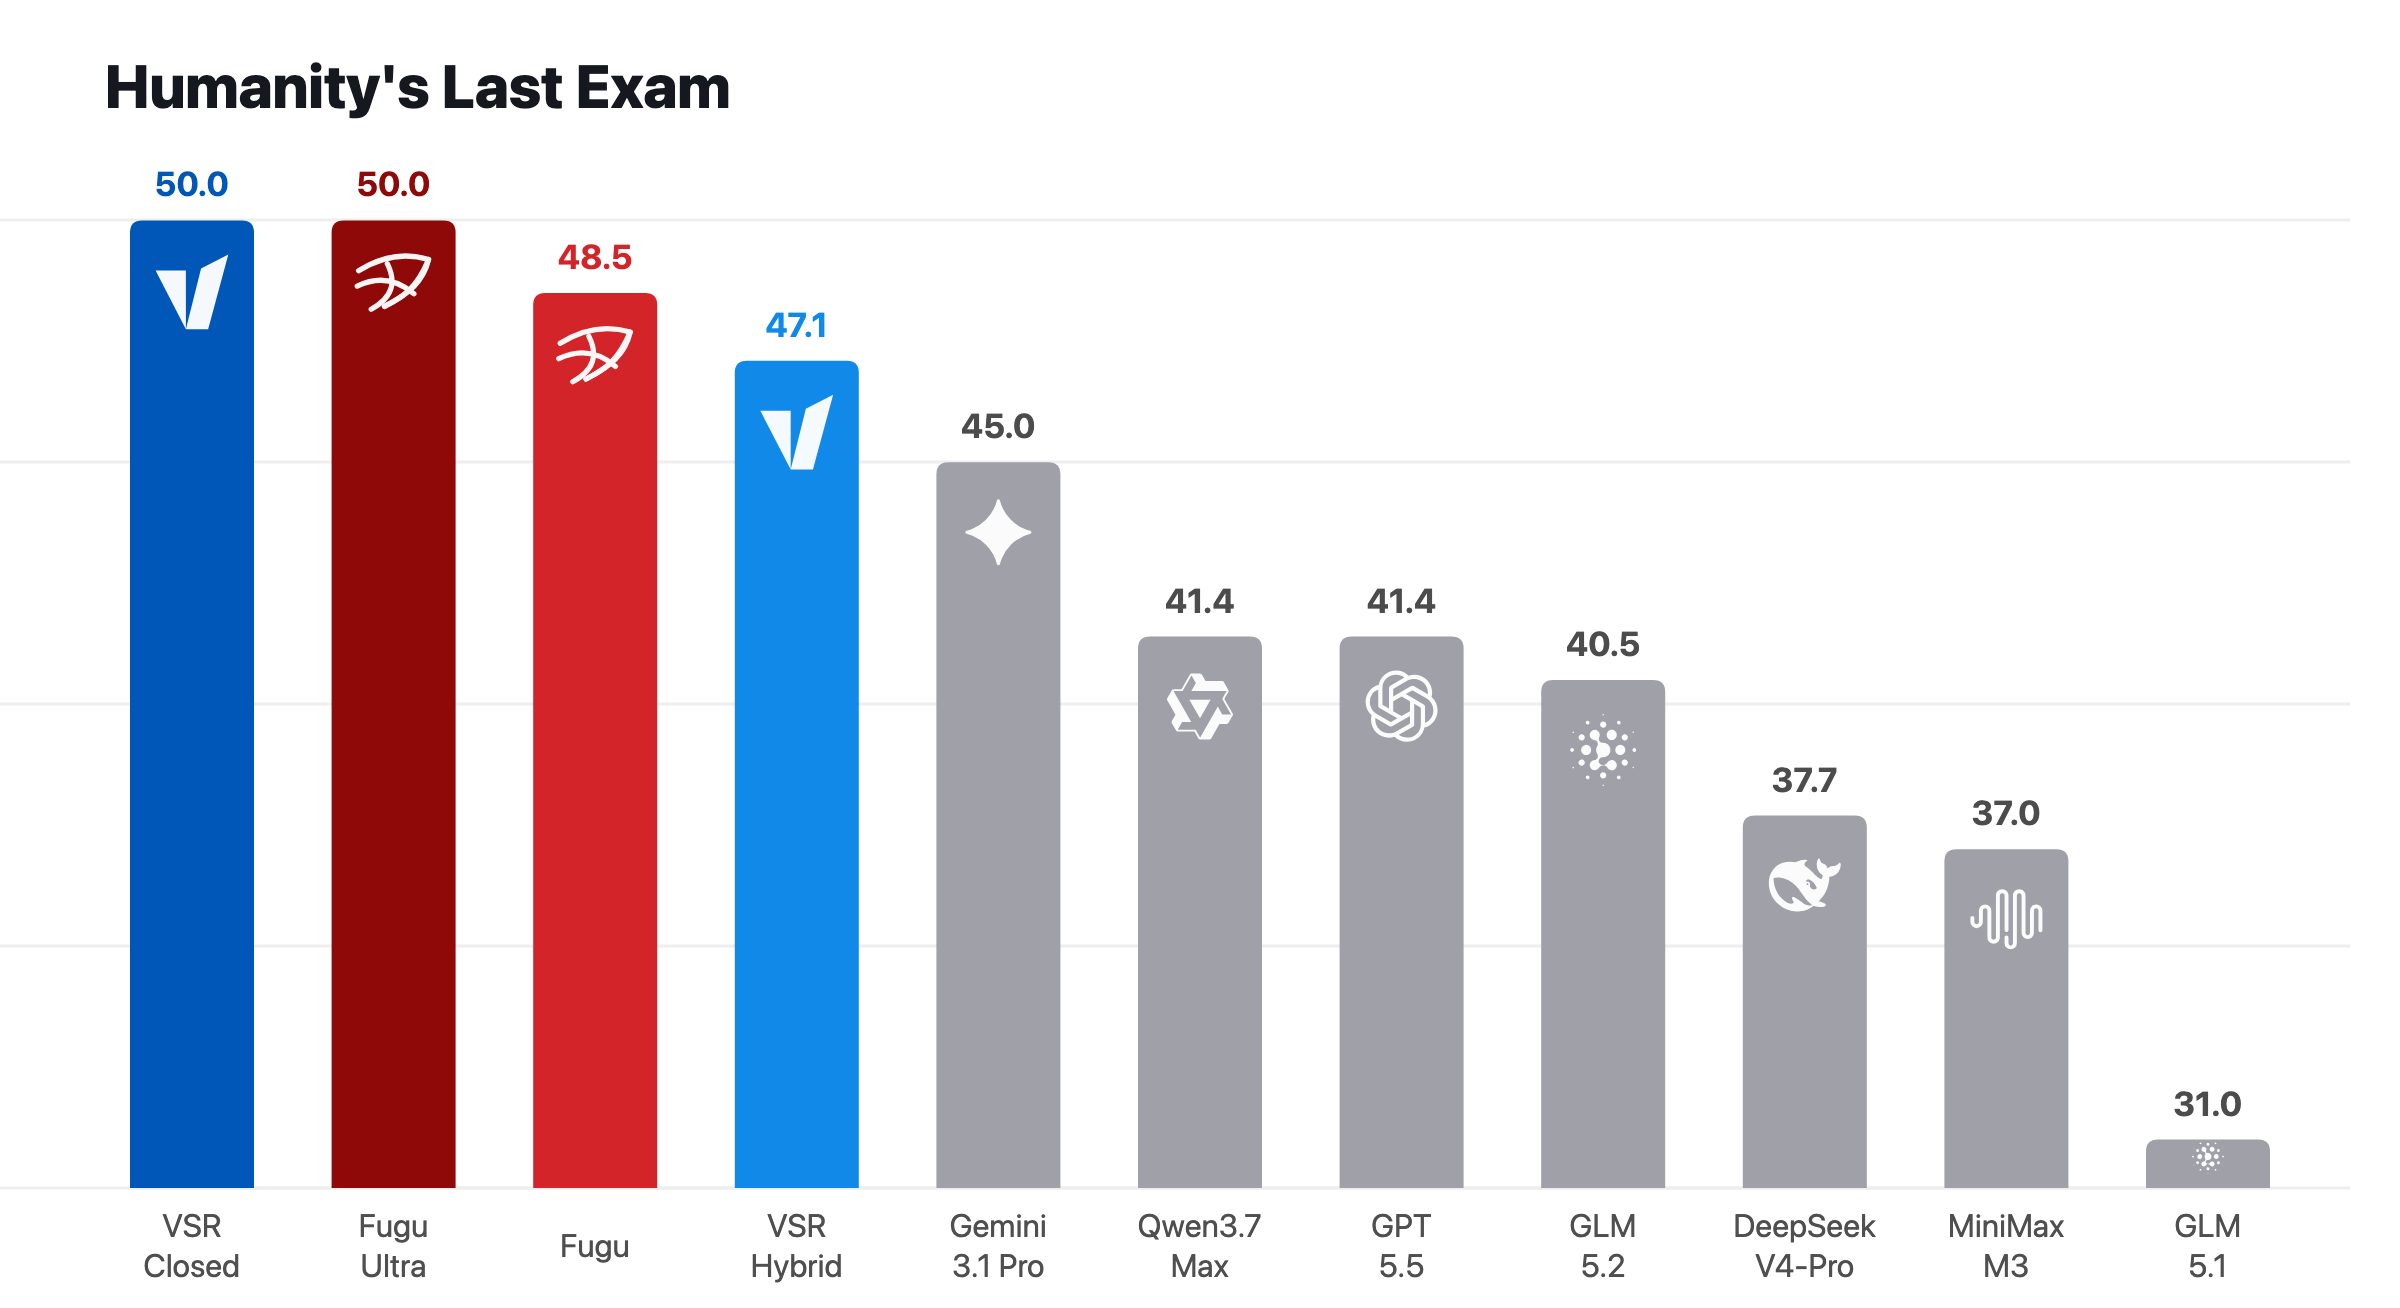
\includegraphics[width=0.27\paperwidth,trim=0 0 1080bp 0,clip]{figures/fig7_hle_scorecard.png}%
  }
  \caption{\textbf{Leading entries from the released accuracy-first MoM
  scorecards.} \emph{VSR Closed} denotes a realization using closed
  constituents; \emph{VSR Hybrid} combines open and closed constituents. GPQA
  uses the formal-50 slice, LiveCodeBench the 175-item January--April 2025
  slice, and HLE a 2,158-item text-only filter. These are protocol-specific
  release snapshots, not a matched-budget comparison
  \citep{vllm_sr_2026_microagent,tang_2026_fugu_v1}.}
  \label{fig:accuracy-scorecards}
\end{figure}

These runs exercise bounded deliberation and synthesis rather than the entire
action algebra. Looper metadata records models used and call counts. Router
Replay and usage records provide aggregate decision, token, and cost data,
while runtime metrics provide latency observability. The canonical per-call
event trace required for strict matched-budget comparison is part of the
proposed evaluation contract.

Figure~\ref{fig:accuracy-scorecards} reproduces the broader scorecard context in
which the results were released. It also includes prior project-reported HLE
closed and hybrid aggregates over a 2,158-item text-only filter
\citep{phan_2026_hle}. Those HLE rows are retained as a released system snapshot;
the current versioned evaluation manifest covers GPQA and LiveCodeBench. Public
reference bars use source-specific protocols and provide context, not a
matched-budget baseline. In particular, the LiveCodeBench and text-only HLE
comparators are pinned to the 175-item and 2,158-item protocols reported with
Fugu v1 rather than the later full-benchmark revision
\citep{tang_2026_fugu_v1}. The figure therefore illustrates that MoM admits an
accuracy-first operating point; it is not the controlled scaling comparison.

\FloatBarrier
\subsection{Routing-aware fleet planning}

Logical routing changes the workload presented to the serving fleet. To
illustrate the connection, an analytical two-pool planner replays the
request-length distribution from LMSYS-Chat-1M, a real-world conversation
dataset collected partly through Chatbot Arena
\citep{zheng_2023_lmsyschat,chiang_2024_chatbotarena}, at 100 requests per
second. The homogeneous estimate assigns all traffic to a 65K-context 70B
profile and yields 14 A100 GPU-equivalents of continuous capacity. A
length-aware split between 4K- and 65K-context pools estimates 8 A100
GPU-equivalents under the same 500 ms time-to-first-token target. At the
planner's assumed \$2.21 per GPU-hour, annualized cost changes from
approximately \$271K to \$155K, a 42.9\% simulated reduction.

This case study instantiates Workload--Router--Pool coupling: the trace policy
shapes the demand seen by each pool, so capacity planning cannot be an
afterthought to model selection \citep{chen_2026_wrp}. Once routing probabilities
and context requirements are explicit, placement and capacity become
optimization variables rather than hidden endpoint properties. The numbers are
analytical capacity estimates, not a production-cluster measurement;
deployment studies must calibrate the planner and repeat the comparison across
hardware, providers, and failure conditions.

\FloatBarrier
\subsection{The controlled scaling test}
\label{sec:required-experiments}

The controlled scaling experiment fixes a benchmark and constructs nested pools
of increasing size and capability diversity. At each size, it compares the
strongest constituent, learned selection, a fixed panel, an adaptive MoM, and an
oracle selector under matched call, token, cost, or latency budgets. It reports
oracle headroom, controller realization, per-item error correlation, topology
activation, contract failures, and repeated-run uncertainty. This design
separates conditional capacity from the effect of spending more inference
compute. Section~\ref{sec:limitations} extends the test to portability,
adaptation, sovereignty, and governance. Figure~\ref{fig:matched-budget-protocol}
summarizes the comparison.

\begin{figure}[H]
  \centering
  \resizebox{\linewidth}{!}{\begin{tikzpicture}[
  x=1cm,y=1cm,font=\sffamily,>=Latex,
  flow/.style={-{Latex[length=2.0mm]},draw=MoMGray,line width=0.70pt},
  group/.style={draw=MoMBorder,fill=MoMBlueLight!10,rounded corners=4pt,
    line width=0.65pt},
  card/.style={draw=MoMBorder,fill=white,rounded corners=2.2pt,
    line width=0.55pt,minimum height=0.52cm,inner xsep=5pt,align=center,
    font=\sffamily\fontsize{6.8}{7.6}\selectfont,text=MoMText},
  core/.style={draw=none,fill=MoMDark,text=white,rounded corners=3pt,
    minimum height=1.15cm,inner xsep=8pt,align=center},
  active/.style={card,draw=MoMDark,fill=MoMBlue,line width=0.72pt},
  oracle/.style={card,draw=MoMDark,fill=MoMPurple,line width=0.68pt},
  title/.style={font=\sffamily\bfseries\fontsize{7.5}{8.3}\selectfont,
    text=MoMText},
  muted/.style={font=\sffamily\fontsize{6.2}{7.0}\selectfont,text=MoMMuted}
]

% One left-to-right evaluation protocol. No curve is shown because this is a
% measurement design, not an empirical result.
\draw[group] (0.00,0.20) rectangle (3.45,3.15);
\node[title] at (1.725,2.88) {Nested catalogs};
\node[card,minimum width=2.55cm] at (1.725,2.25)
  {Catalog 1\quad base models};
\node[card,minimum width=2.55cm] at (1.725,1.58)
  {Catalog 2\quad + specialist};
\node[card,text width=2.25cm,minimum height=0.64cm] at (1.725,0.91)
  {Catalog 3\\+ modality / provider};
\node[muted] at (1.725,0.43)
  {nested by inclusion};

\node[core,minimum width=2.70cm] (budget) at (5.30,1.68)
  {{\bfseries\fontsize{8.0}{8.8}\selectfont Same active budget}\\[-1pt]
   {\fontsize{6.5}{7.2}\selectfont bounded calls \textbullet\ bounded tokens}\\[-1pt]
   {\fontsize{6.2}{6.9}\selectfont cost or latency matched}};

\draw[group] (7.20,0.20) rectangle (11.92,3.15);
\node[title] at (9.56,2.88) {Compared policies};
\node[card,minimum width=1.62cm] at (8.17,2.23) {strongest};
\node[card,minimum width=1.62cm] at (9.94,2.23) {selection};
\node[card,minimum width=1.62cm] at (11.02,1.55) {fixed panel};
\node[active,minimum width=1.90cm] at (8.48,1.28) {adaptive MoM};
\node[oracle,minimum width=1.62cm] at (10.45,0.72) {oracle};

\draw[group] (12.68,0.20) rectangle (16.30,3.15);
\node[title] at (14.49,2.88) {Report};
\node[card,minimum width=2.72cm] at (14.49,2.18) {oracle headroom};
\node[card,minimum width=2.72cm] at (14.49,1.50) {controller realization};
\node[card,minimum width=2.72cm] at (14.49,0.82)
  {error correlation / activation};

\draw[flow] (3.45,1.68) -- (budget.west);
\draw[flow] (budget.east) -- (7.20,1.68);
\draw[flow] (11.92,1.68) -- (12.68,1.68);

\end{tikzpicture}
}
  \caption{\textbf{Matched-budget protocol for MoM scaling.} Nested catalogs
  are evaluated under one active-work envelope. Comparing a strongest
  constituent, learned selection, a fixed panel, an adaptive MoM, and an oracle
  separates catalog complementarity from controller realization and additional
  inference work. The diagram specifies an evaluation protocol, not a result.}
  \label{fig:matched-budget-protocol}
\end{figure}

\FloatBarrier
